\documentclass[a4paper]{article}
\usepackage[fleqn]{amsmath}
\usepackage{graphicx}
%\usepackage{times}
\usepackage[framed,numbered,autolinebreaks,useliterate]{mcode}
\usepackage{listing}
\usepackage[small,compact]{titlesec}
\usepackage[utf8]{inputenc}

\usepackage{biblatex}
\bibliography{../Documentation.bib}

\usepackage[paper=a4paper,
            includefoot, % Uncomment to put page number above margin
            marginparwidth=30.5mm,    % Length of section titles
            marginparsep=1.5mm,       % Space between titles and text
            margin=10mm,              % 25mm margins
            includemp]{geometry}

%\setlength{\oddsidemargin}{10mm}
%\setlength{\evensidemargin}{10mm}
\usepackage{fullpage}

\usepackage{multicol}
\usepackage{caption}

\newcommand{\makeheading}[2]%
        {\hspace*{-\marginparsep minus \marginparwidth}%
         \begin{minipage}[t]{\textwidth\marginparwidth\marginparsep}%
           {\large \bfseries #1}\\{#2}\\[-0.15\baselineskip]%
                 \rule{\columnwidth}{1pt}%
         \end{minipage}}

\newlength{\figurewidth}
\setlength{\figurewidth}{500px}


\begin{document}
\makeheading{Gautebøye - Instrument Response}{Gaute Hope
(gaute.hope@student.uib.no), 29.05.2012, Revision 2 (12.08.2012)}

\vspace{2em}
\section*{Introduction}
Here is presented the theoretical derivation and analysis of the analog
instrument response of the digitizer. The digital filtering during AD
conversion is briefly discussed, but its properties are well defined in
the manual of the ADC\cite{ads1282_ds}. \vspace{2em}

\begin{multicols}{2}
\section{Hydrophone decoupling}
\end{multicols}
\begin{center}
  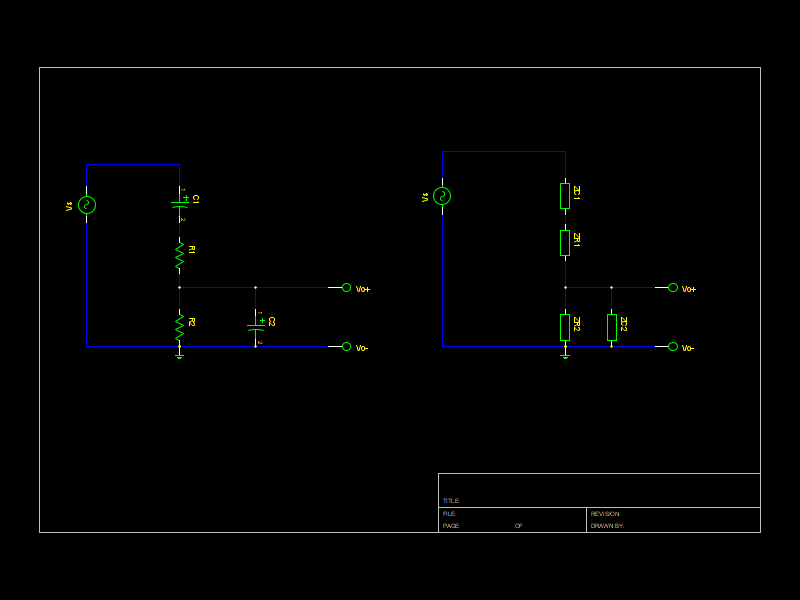
\includegraphics[width=400px]{Hydrophone_decoupling.png}
  \captionof{figure}{Hydrophone decoupling circuit}
  \label{fig:hydrophone_decoupling}
\end{center}

\begin{multicols}{2}
The figure above (\ref{fig:hydrophone_decoupling}) shows an equivalent
circuit of the deployed input decoupling to the hydrophone.


\begin{align*}
  C_1 &= 47 \mu F \\
  C_2 &= 330 pF \\
  R_1 &= 58.33 k \Omega \\
  R_2 &= 41.67 k \Omega
\end{align*}

\paragraph{}The circuit was based on the suggested decoupling in figure
\ref{fig:suggested_decoupling} seen below, it was designed to have the
same properties, but also low-pass the signal at cutoff frequency
$f_{LP_1}$. The original design already decouples, and high-passes, the
signal at frequency $f_{HP}$.

  \begin{center}
    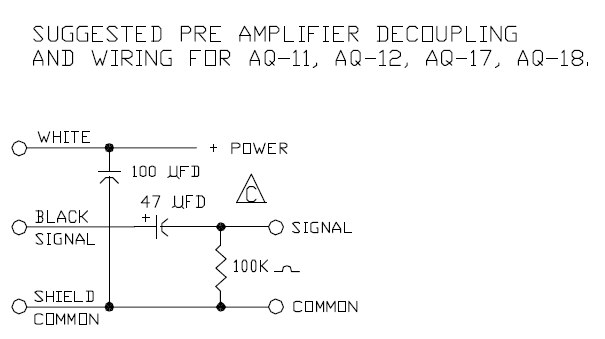
\includegraphics[width=200px]{AQ-18-decoupling-and-wiring.jpg}
  \end{center}
  \captionof{figure}{AQ-18 suggested decoupling and wiring
    \cite{aq-18_decoupling}.}
  \label{fig:suggested_decoupling}

\section{Derivation of transfer function}

$i_1$ and $i_2$ signify the current loops passing through respectively left
and right loop. Using Kirchoff's equation:

\begin{align}
  \label{eqn:currents_1}
  V_s &= i_1 (Z_{C_1} + Z_{R_1}) + (i_1 - i_2) \cdot Z_{R_2} \\
  0   &= (i_2 - i_1) \cdot Z_{R_2} + i_2 \cdot Z_{C_2}
  \label{eqn:currents_2}
\end{align}

$V_s$ is the signal source, the hydrophone. See separate data sheet for
hydrophone frequency response. $V_o$, output, is measured at the
terminals $T_+$ and $T_-$.

\begin{align}
  \label{eqn:vo}
  V_o &= i_2 \cdot Z_{C_2} \\
  H(s) &= \frac{V_o}{V_s}, s = i\omega
\end{align}

Solving for $H(s)$ gives:

\begin{equation}
  H(s) = \frac{51951 s}
  { (s + 1.2470 \times 10^5)
    (s + 0.2128) }
  \label{eqn:transferfunction}
\end{equation}

A bode plot of the transfer function (instrument response) is shown in
figure \ref{fig:bodeplot} below.

\end{multicols}
  \begin{center}
    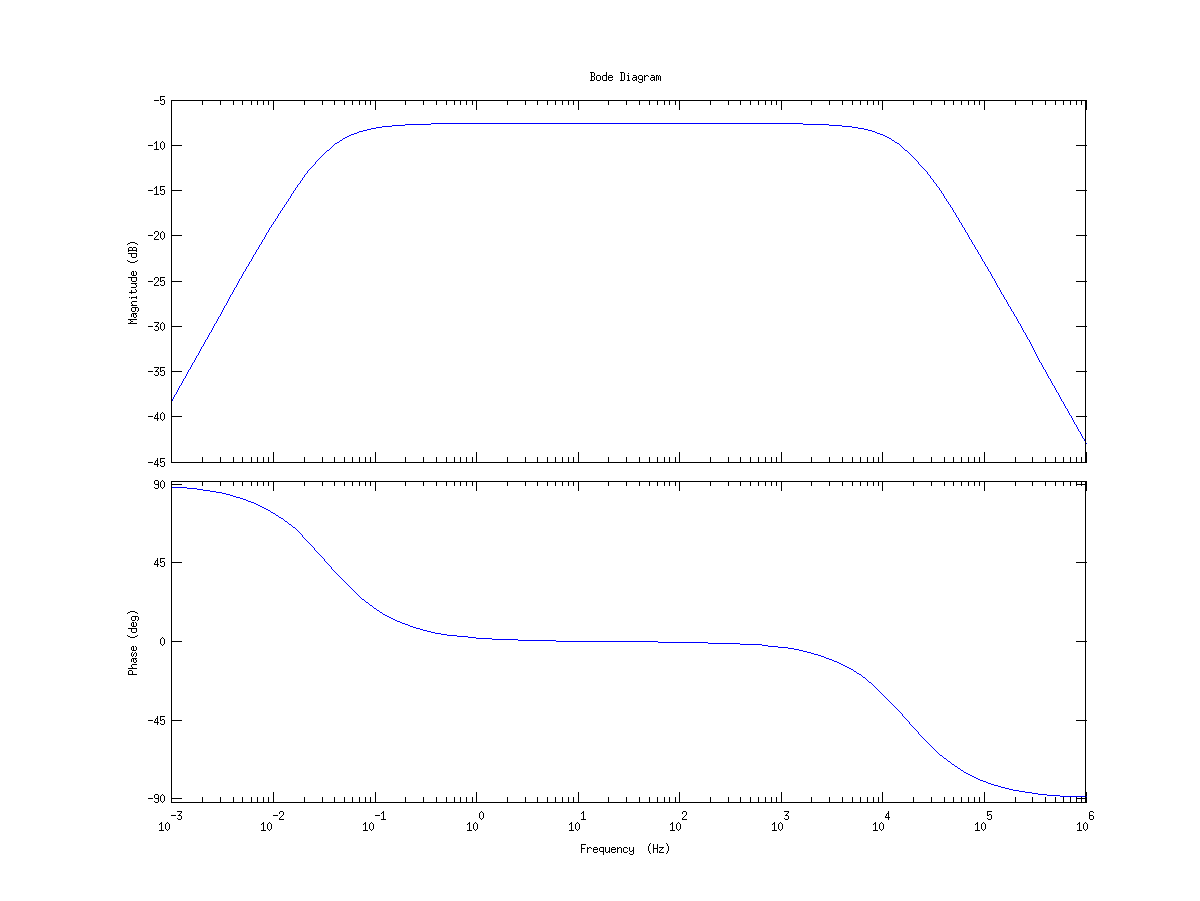
\includegraphics[width=400px]{bodeplot.png}
  \end{center}
  \captionof{figure}{Bode plot of transfer function, showing peak response at
  $33.9$ Hz.}
  \label{fig:bodeplot}

\begin{multicols}{2}
Equation \ref{eqn:transferfunction} can be solved by using the MATLAB
script response.m (listing \ref{code:response_m}), the Bode plot in figure \ref{fig:bodeplot} was created with the same script.

\subsection{Analysis}
The initial frequency band of interest reaches
from periods of 20 s (0.05 Hz) to approximately $100$ Hz. The analog input part as
well as the configuration of the analog-digital converter has been
configured to as best and simple as possible to record the signal
within this frequency band.

\subsubsection{Decoupling and analog high pass filter}
The transfer function is a bandpass filter with
the suggested decoupling creating a high-pass filter with corner
frequency at $f_{HP} = 0.0339$ Hz or a period of $29.4985$ s.

\subsubsection{Low pass filter and operational amplifier}

To avoid aliasing due to the speed of the opamps (operational
amplifiers) in the signal path; the OPA627 (see \cite{opa627_ds} and
figure \ref{fig:hydrophone_decoupling}) acting as buffer with
unity gain and then the OPA1632 \cite{opa1632_ds} at the input terminals
of the ADS1282EVM \cite{ads1282evm_ds}.
An additional low pass stage is added with a corner frequency of
$f_{LP_1} = 17.189 $ kHz. The speed of the opamp is in the order of Mhz
so this corner frequency should be well within their capabilities.

\paragraph{OPA1632} \ \\
The OPA1632 \cite{opa1632_ds} is set up with a 1 nF capacitor in its
feedback loop on the ADS1282EVM \cite{ads1282evm_ds}, this low passes
the signal with an cut off frequency at $f_{LP_2} = 151.99$ kHz. Its
gain bandwidth is specified to be 180 MHz, given that the gain is 1 and
the load is large it should have a well behaved and near ideal response. The
OPA1632-setups simplified transfer function is \cite{fully_diff_opamps}:

\begin{equation}
  H_{OPA1632}(s) = \frac{9.551 \times 10^5}
                        {(s + 9.551 \times 10^5)}
  \label{eqn:opa1632_tf}
\end{equation}

\paragraph{OPA627} \ \\
The OPA627 is used as a buffer with gain 1 to provide a high impedance input and low
impedance output. It has a gain bandwidth product of 16 MHz at this
gain \cite{opa627_ds}. With the first low pass filter, $f_{LP_1}$, well
below this it should be able to relay the signal without problems. The
transfer function would simply be 1 for this step. It is important that
the OPA627 has well mounted bypass capacitors to avoid oscillations when
configured for this low gain. An buffer designed for unity gain, like
the OPA633 \cite{opa633_ds} or BUF634 \cite{buf634_ds} could prove a better choice.

\paragraph{OPA633} \ \\
The OPA633 \cite{opa633_ds} is a strong candidate for an drop-in replacement of the
OPA627, it is specifically designed to be a buffer working at unity
gain. The feedback loop is internally connected. But otherwise the same
wiring scheme applies. Closely mounted and well chosen bypass capacitors
are still needed on the power supplies to ensure stability. The input
impedance of the ADS1282EVM should be sufficient for the gain to
approach unity. The OPA633 has a gain bandwidth of 260 MHz, however it
requires $\pm 15$ mA current, which is about twice that of the OPA627.

\subsubsection{Stability}
The system, $H(s)$ from equation \eqref{eqn:transferfunction}, is
passive and has all
its poles in the left half plane and is stable.

\subsubsection{Analog-Digital Converter (ADC)}
The ADS1282EVM equips its ADS1282 with a crystal with the recommended clock frequency of
$f_{clk} = 4.096$ Mhz \cite{ads1282evm_ds}. This results in a modulator
output speed of $ f_s = f_{clk}/4 = 1.024$ Mhz \cite{ads1282_ds}. The
Nyquist frequency is then:

\begin{equation}
  f_{Nq} = 1.024 \times 10^6 / 2 = 512\ \text{kHz}
  \label{eqn:nyquist}
\end{equation}

\end{multicols}

  \begin{center}
    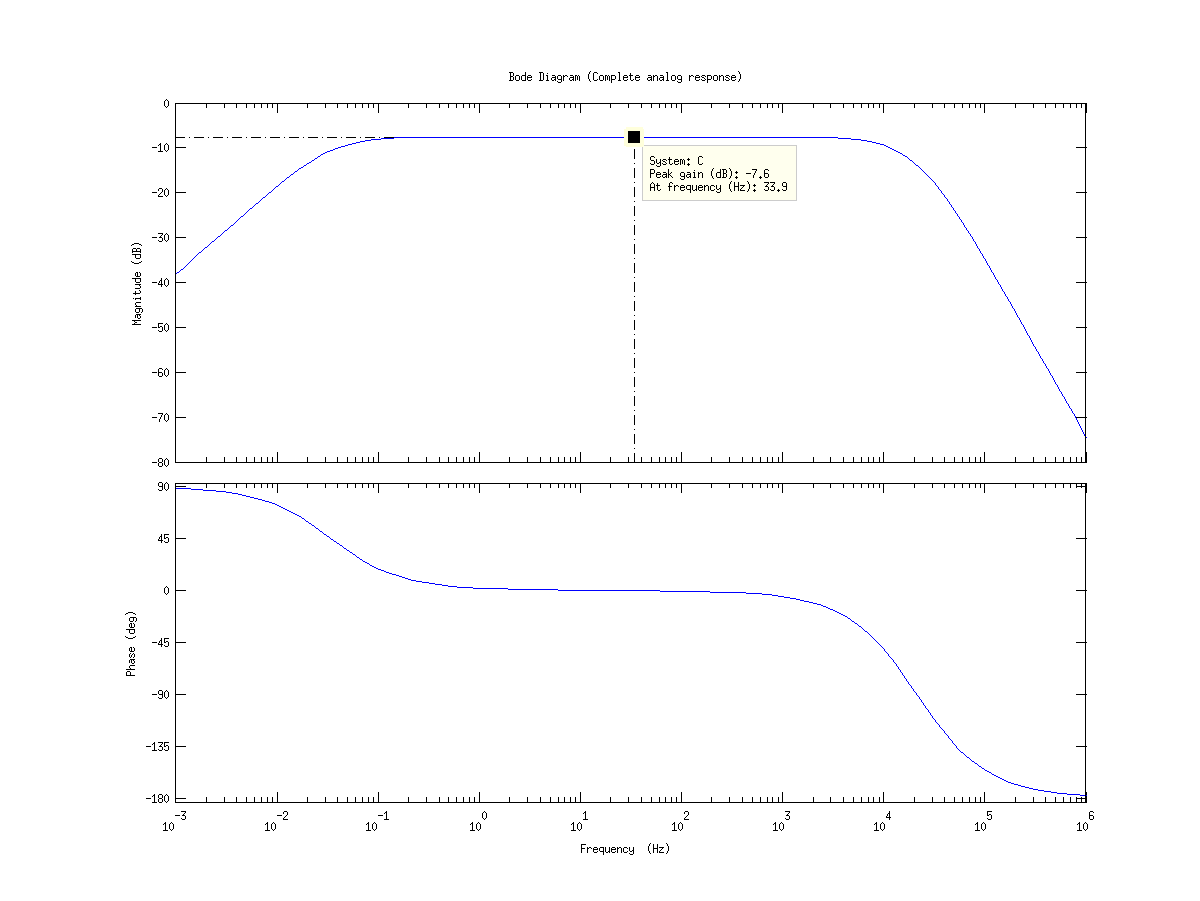
\includegraphics[width=400px]{bode_complete_analog.png}
  \end{center}
  \captionof{figure}{Frequency response of complete analog system, equation
    \eqref{eqn:transfer_analog}.}
  \label{fig:bode_complete_analog}

  \begin{multicols}{2}

\subsubsection{Anti-alias filter}
The 10 nF capacitor used on the ADS1282EVM
\cite{ads1282evm_ds}, results in a low-pass filter with an upper corner frequency of $f_{LP_3} =
\frac{1}{2 \pi \times 600 \times 10 \times 10^{-9}} = 26525.82 $ Hz
\footnote{Equation (3), p.15, \cite{ads1282_ds}; \citetitle{ads1282_ds}}.

$f_{LP_3}$ is thus well below $f_{Nq}$ and any signal component above $f_{LP_3}$ should
be almost completely damped before it reaches $f_{Nq}$, resulting in no
or very small aliasing effects.

This equation represents the upper low pass filter:
\begin{center}
\begin{equation}
  \begin{aligned}
  H_{UL}(s) &= \frac{1 \div 600 \times 10 \times 10^{-9}}
                   {(s + 1 \div 600 \times 10 \times 10^{-9})} \\
            &= \frac{1.667 \times 10^5}{(s + 1.667 \times 10^5)}
  \end{aligned}
  \label{eqn:transfer_upper_lowpass}
\end{equation}
\end{center}

The complete analog transfer function is then:
\begin{center}
\begin{equation}
  \begin{aligned}
  H_{a} = &\frac{8.2698 \times 10^{15}}
                { (s + 9.551 \times 10^5) \times
                   (s + 1.667 \times 10^5)
                 } \times \\
          & \frac{1}
                 {(s + 1.247 \times 10^5) \times
                  (s + 0.2128) }
  \end{aligned}
  \label{eqn:transfer_analog}
\end{equation}
\end{center}


The frequency response is illustrated in figure
(\ref{fig:bode_complete_analog}).
\subsubsection{Output of decoupling and buffer} The output is scaled by $-7.6\ \text{dB} =
0.4169 \frac{V}{V}$ which is to scale the input from $\pm 6V$ to $\pm 2.5V$, $0.4169
\approx 5 / 12 = 0.4167$, which is the input range of the ADS1282EVM
(\cite{ads1282evm_ds} and \cite{ads1282_ds}) in bipolar mode. The
slightly inaccurate scaling is due to the available (high precision) resistor values.

\paragraph{}
The impulse response of the system is plotted in figure
\ref{fig:impulse_complete_analog}:

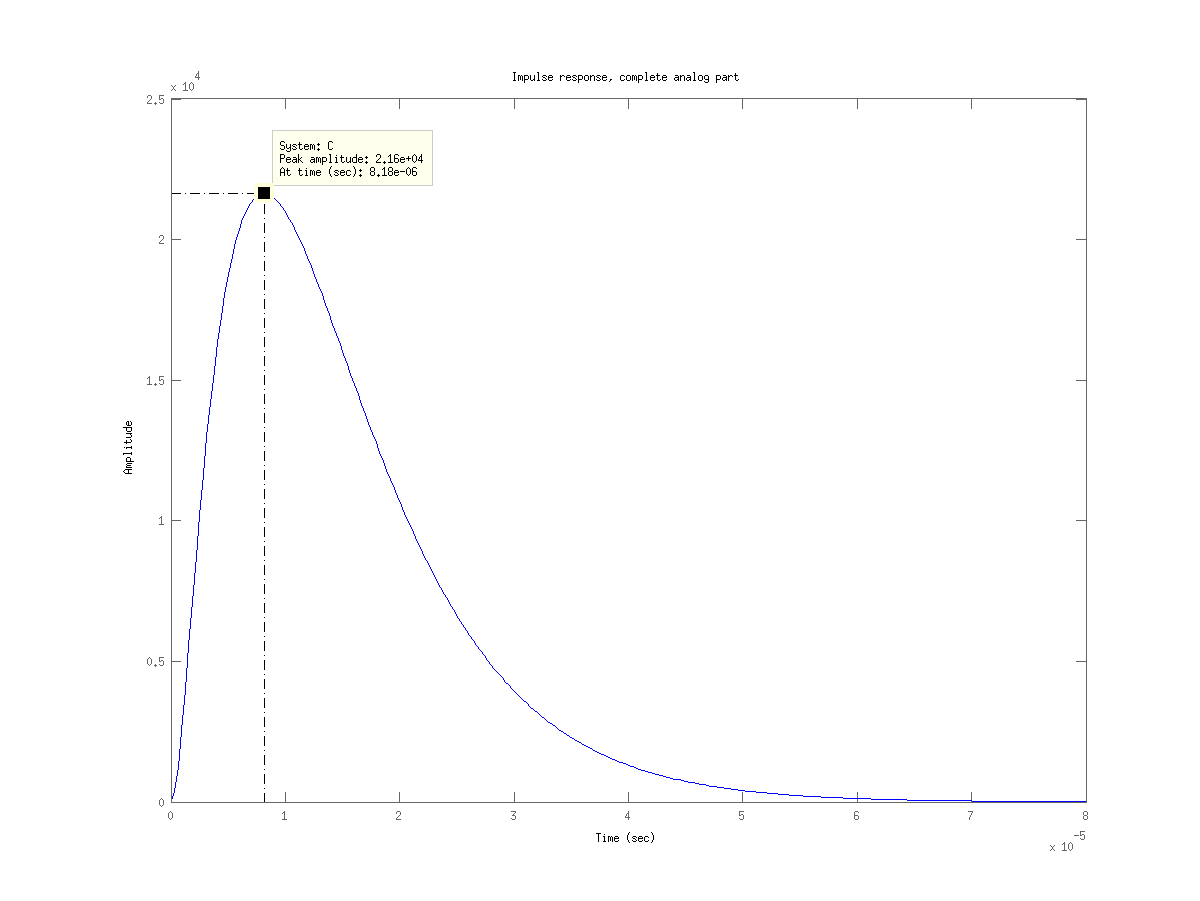
\includegraphics[width=220pt]{impulse_complete_analog.png}
\captionof{figure}{Impulse response of complete analog system, equation
  \eqref{eqn:transfer_analog}.}
\label{fig:impulse_complete_analog}

\paragraph{}
The step response, large is plotted in figure
\ref{fig:step_complete_analog}:
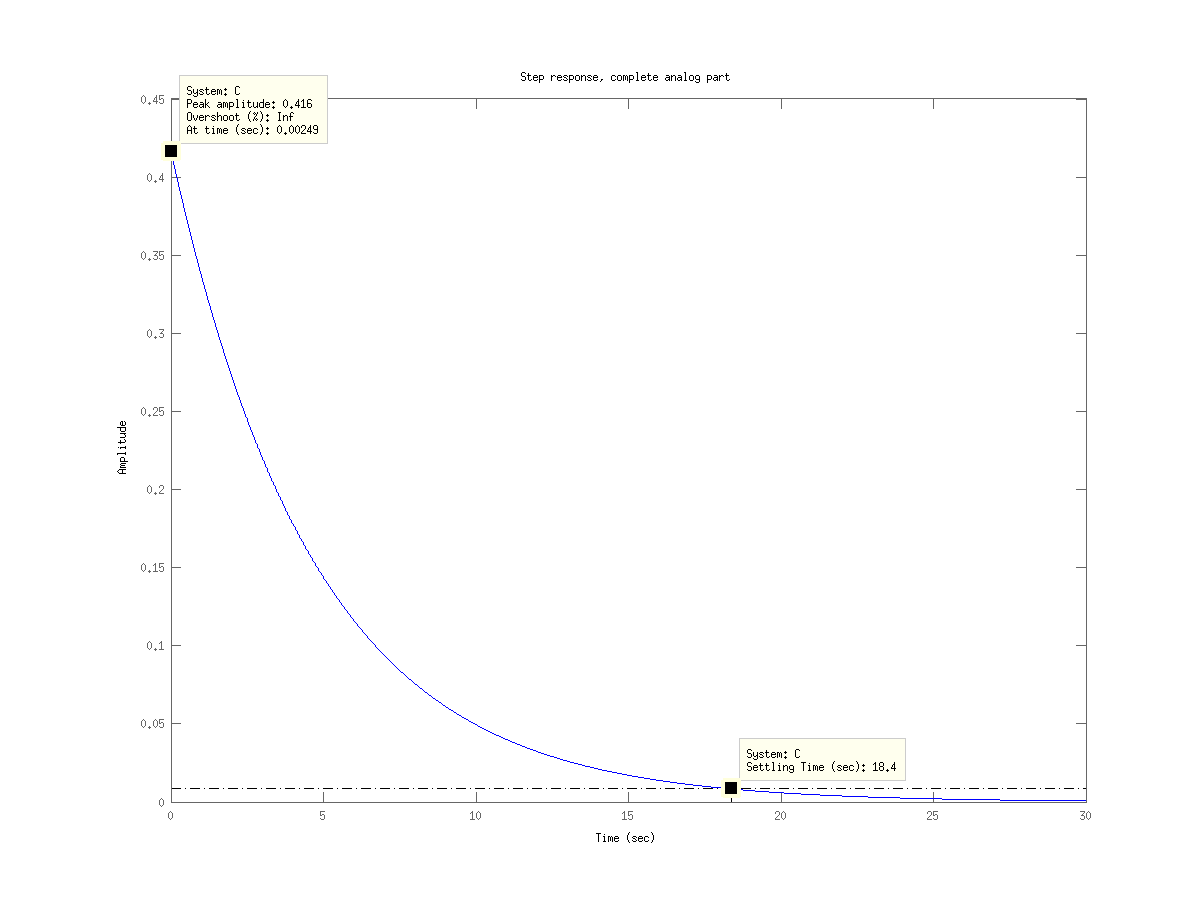
\includegraphics[width=220pt]{step_complete_analog.png}
\captionof{figure}{Step response of complete analog system, equation
  \eqref{eqn:transfer_analog}.}
\label{fig:step_complete_analog}

\paragraph{}
A zoomed in section of the high frequency response is shown in figure
\ref{fig:step_zoom_complete_analog}, the first tens of microseconds.
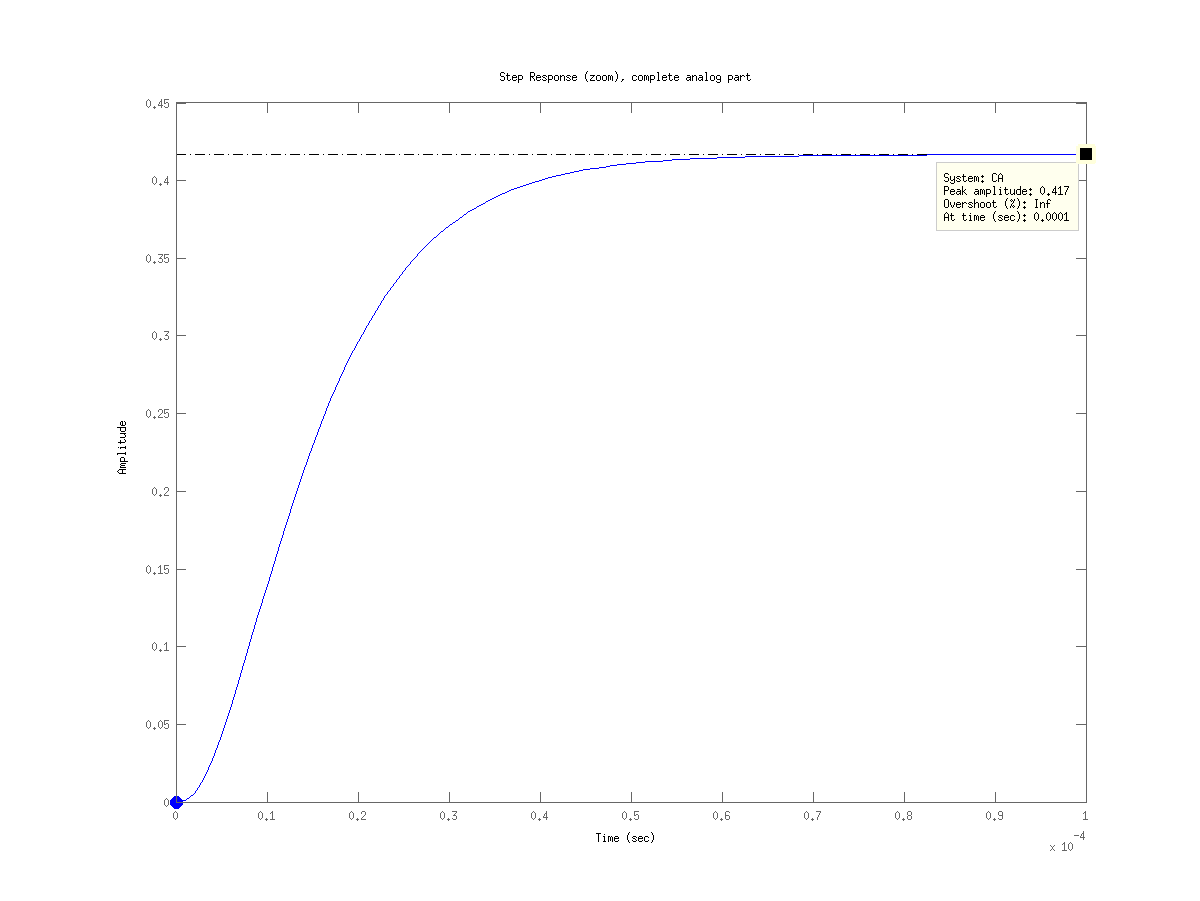
\includegraphics[width=220pt]{step_zoom_complete_analog.png}
\captionof{figure}{Step response (zoomed) of complete analog system, equation
  \eqref{eqn:transfer_analog}.}
\label{fig:step_zoom_complete_analog}

\paragraph{Attenuation at Nyquist frequency}\ \\
The attenuation at the Nyquist
frequency, $512$ kHz, equation \eqref{eqn:nyquist} using
\eqref{eqn:transfer_analog}, is evaluated to be:
\begin{equation}
  \begin{aligned}
  | H_a(512 \times 10^3 \times 2 \pi) | &= 0.00023763 \\
                                        &= -72.4821\ \text{dB}
  \end{aligned}
  \label{eqn:attenuation_nyquist}
\end{equation}

The theoretical maximum dynamic range is specified to be 130
dB\footnote{Table 1, p. 13, \cite{ads1282_ds}; \citetitle{ads1282_ds}}.
But before reaching the frequencies of any signals not attenuated at
\eqref{eqn:attenuation_nyquist} that wraps around to the 125 Hz passband of
the digital filter (section \ref{digitalfilter}) they will be additionally
attenuated. The next periods will be increasingly attenuated.
\paragraph{} Depending on the noise spectra there will
be only a fraction of the noise that is in this passband. Any tones or
oscillations from the electrical components or environment are, although
unlikely to be entirely in this passband, the biggest worry. Other noise
is likelier to have a flatter spectra, where only a fraction of its
amplitude will wrap into the 125 Hz passband.


\label{digitalfilter}
\section{Digital filter}
Further the ADS1282 is configured to digitally filter the decimation
output so that the final output signal of 250 Hz contains no alias below
the input Nyquist sample rate (equation \eqref{eqn:nyquist}). The
built-in sinc and FIR filters are activated, see the ADS1282 datasheet
\cite{ads1282_ds} for details. This provides more
than $140$ dB of attenuation above the Nyquist frequency of the output
sample rate \cite{ads1282_ds}.
\paragraph{}The
ADS1282 can be configured for an sample rate of as high as 4000 Hz
\cite{ads1282_ds}. This would be possible without changes in the analog
interface, although it would come at an cost of resolution and would
require adaption of the firmware of the buoy to handle the higher data
rate.

\paragraph{High Pass Filter (HPF)} The ADS1282 is configured to have an high
pass corner frequency as close to 20 seconds as possible, the built in
IIR HPF is set according to p. 22 in \citetitle{ads1282_ds}:

\begin{equation}
  \begin{aligned}
    & HPF[1:0] = 65,536 \times \\
    & \left[ 1 - \sqrt{1 - 2 \frac{\cos (\omega_n) +
    \sin (\omega_n) - 1}{\cos
    (\omega_n)}}\right]
  \end{aligned}
  \label{eqn:hpf}
\end{equation}

with:

\begin{equation}
  \omega_n = 2 \pi f_{HP} / f_{DATA}
  \label{eqn:nat_freq}
\end{equation}

An $f_{HP} = 1/20 = 0.05 $ Hz gives an $\omega_n = 0,001256637$ normalized
radians. And an $HPF[1:0] = 82.3550098$ truncated to $HPF[1:0] = 82_{10} =
52_{16}$.

\section{Hydrophone characteristics}
The hydrophone used, Benthos AQ-18, is specified to have an flat frequency response within
$\pm 1.5 \text{dB}$ at the band 1 - 10 kHz
\cite{benthos_hydrophone_brochure}. With a sensitivity of -171 dBv re 1
uPa at $20^\circ$ C. \textbf{TODO:} Need lower corner frequency and
details.. Transfer function for hydrophone:

\begin{equation}
  H_{Hyd} = - 171\ \text{dBv re}\ 1\ \text{uPa} = 10^{8.55}
  \ \frac{\text{V}}{\text{uPa}}
  \label{eqn:transfer_hydrophone}
\end{equation}

\section{Response of Digitizer}
In addition to the digital filters, however very sharp should ideally be
included, the output is 32 bit integers, with a range of $\left[ -2^{31},
  2^{31} - 1 \right]$, disregarding for simplicity (\textbf{FIXME}),
the transfer function for the digitization part is: 

\begin{equation}
  H_{D} = \frac{2^{32}}{5} \frac{\text{counts}}{\text{V}}
  \label{eqn:digital_transfer}
\end{equation}

\section{Response compared to output of a seismometer}
The hydrophone measures pressure (uPa) while the seismometer measures
displacement (nm), to be able to compare these some relation has to be
figured out.

\paragraph{} Considering that a force is exerted proportional to the
pressure the hydrophone is measuring and that acceleration is
proportional to force the easiest is to consider the hydrophone an
accelerometer.

\vspace{5em}
\printbibliography
\end{multicols}

\newpage

\section{Attachments}
\subsection{response.m}
\lstset{caption={response.m, MATLAB code for calculating instrument
response},label=code:response_m}
\lstinputlisting{response.m}


\end{document}

